% Homework 4.tex 

\documentclass{article}
\usepackage{graphicx} % for figures
\usepackage{float}
\usepackage[export]{adjustbox}
\usepackage{fancyhdr}
\begin{document}

\title{Homework 8 - Physics 240\\
		Comet Extraordinair}
\author{Tin Tran}

\maketitle

\section{Introduction}
This is an exercies to calculate and plot the orbit of the Earth in the comic in 3D, as well write the data to a file then plot them together.
For the comet I picked comet Encke as my comet and calculate its circular velocity, from that I obtained the plot below.
\begin{figure}[H]
\centering{
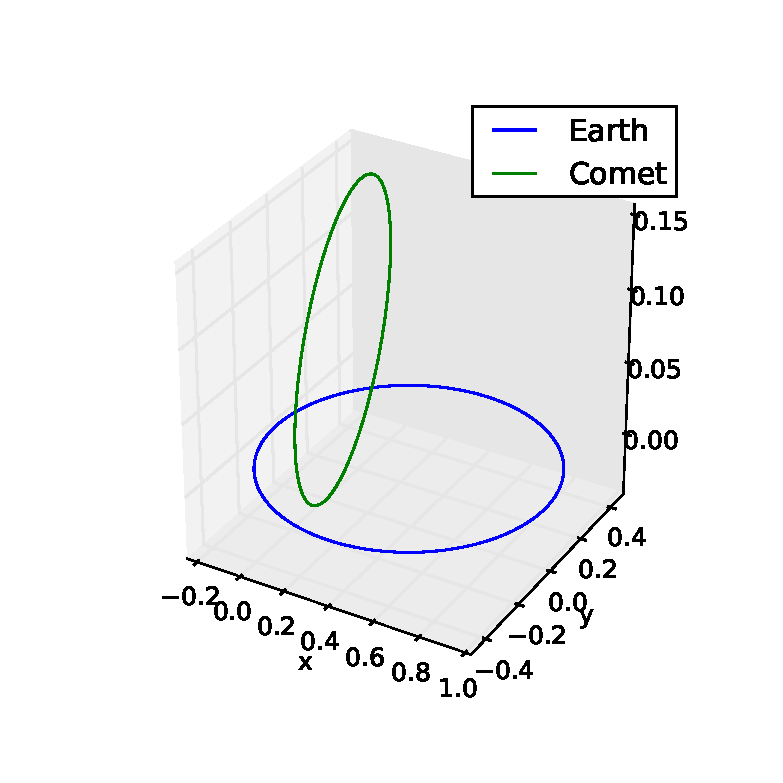
\includegraphics[max size={\textwidth}{\textheight}]{earthcomet.eps}
\caption{Trajector of the Earth and Comet }
}
\end{figure}

After that I added the drag force F$_d$ that I calculated from the equation $|$F$_g$(r$_1$)$|$ = 100$|$F$_d$(v$_1$)$|$ and from that I got the plot below


\section{Introduction}
This is an exercies to calculate and plot the orbit of the Earth in the comic in 3D, as well write the data to a file then plot them together.
For the comet I picked comet Encke as my comet and calculate its circular velocity, from that I obtained the plot below.
\begin{figure}[H]
\centering{
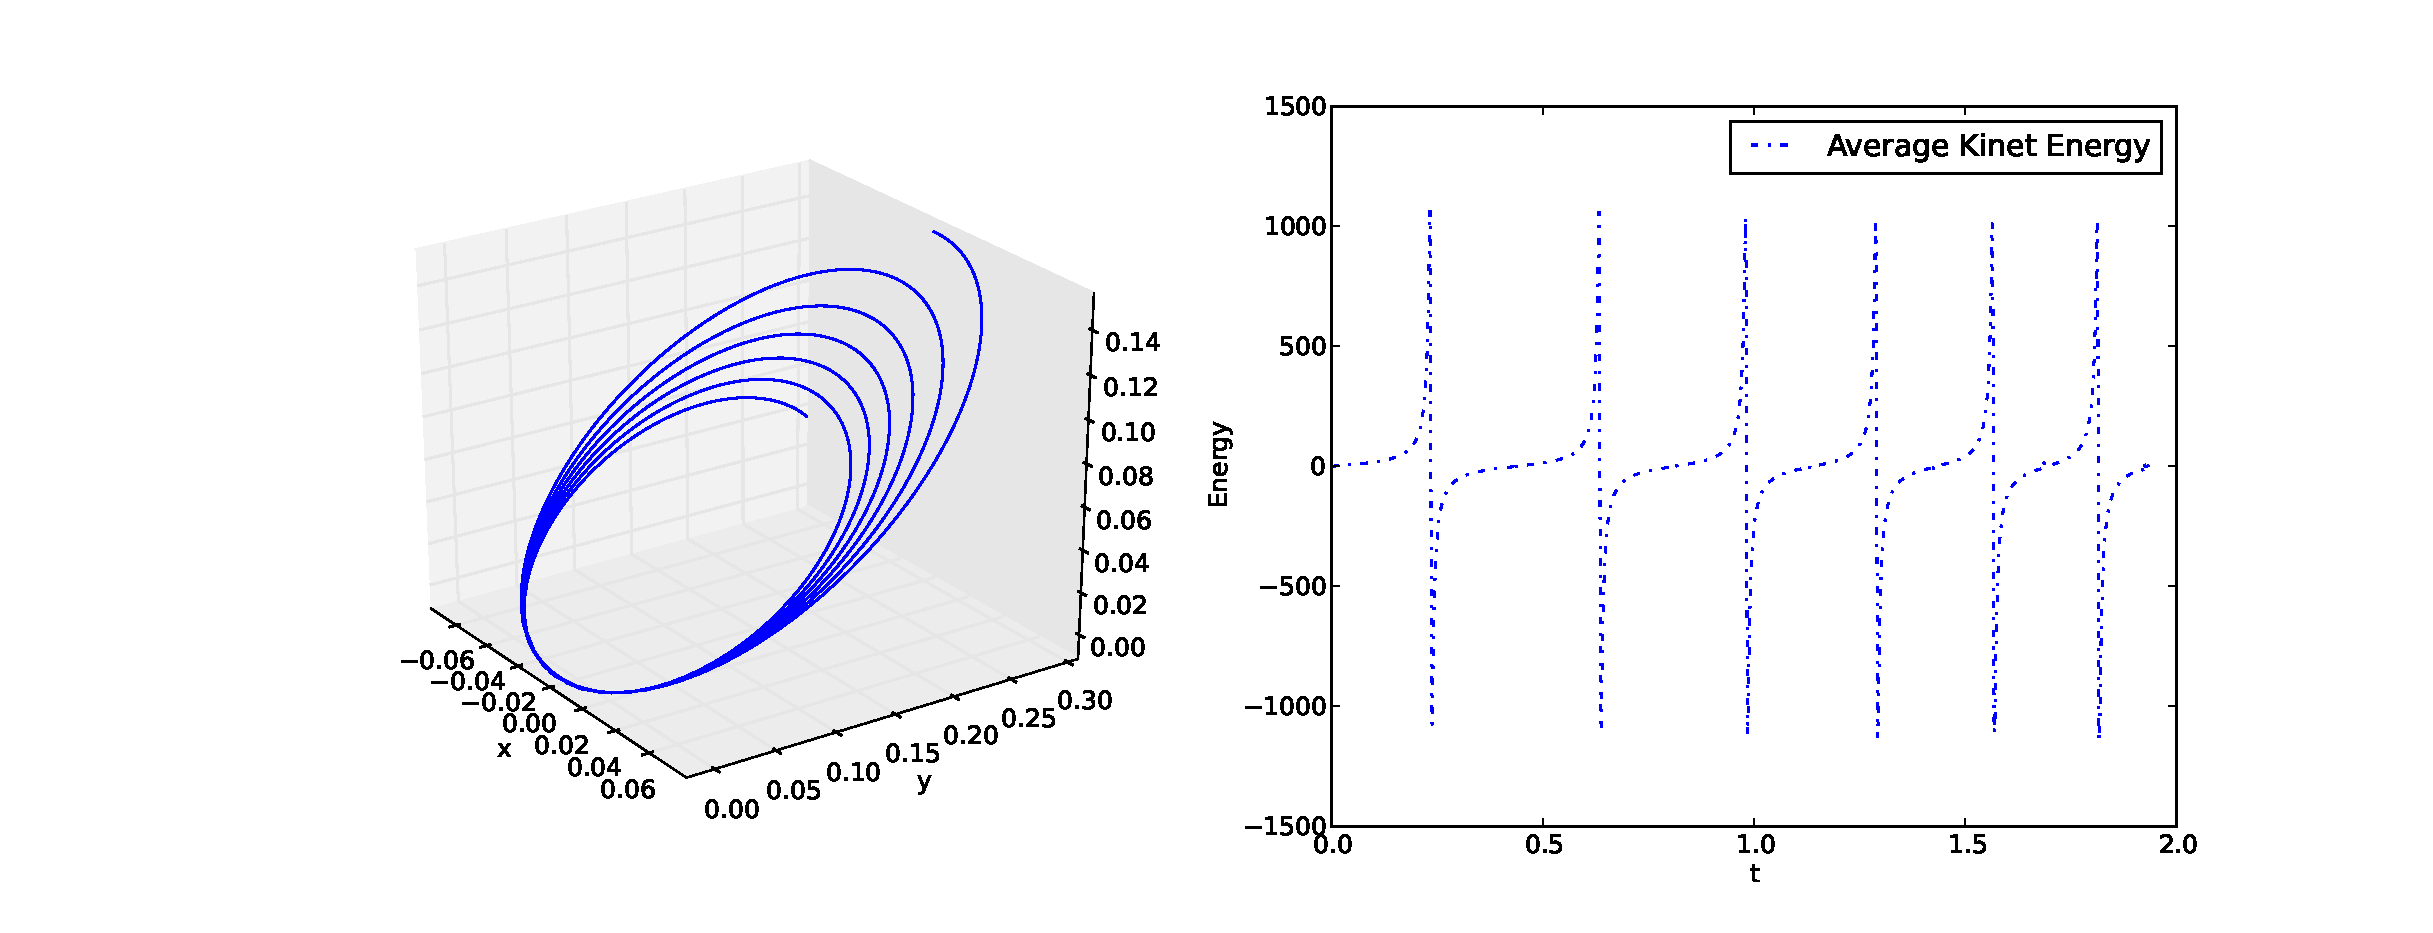
\includegraphics[max size={\textwidth}{\textheight}]{comet.eps}
\caption{Comet trajectory with drag force}
}
\end{figure}

This makes sense to me because the plot shows that for each orbit, the average kinetic energy over an orbit increases with time.kjkl
\end{document}